\documentclass[../primer.tex]{subfiles}

\begin{document}

% --------------------------------------------------
\chapter{Demonstrations}
% --------------------------------------------------
(Here we give a tour of UQ through examples; a la Saltelli's Primer.)

\section{Tricked by Uncertainty `Quantifauxcation'}
% --------------------------------------------------
In this example, we show how the `careless' quantification of uncertainty can
lead to false conclusions. We also motivate the use of forward propagation of
uncertainty, and provide a concrete example of model-form uncertainty.

We consider the buoyancy-driven cavity flow of a viscous fluid, pictured
schematically in Figure \ref{fig:cavity-schematic}.\footnote{This example was
  originally prepared by Dr. Gary Tang.} This is a model problem for studying
the effects of fluid properties on buoyancy-driven flows, with an eye towards
quantifying the uncertainties in climate modeling. Uncertainty arises from the
fluid density-temperature relationship, and our output quantity of interest
(qoi) is the temperature of the bottom wall.

\begin{figure}[!ht]
  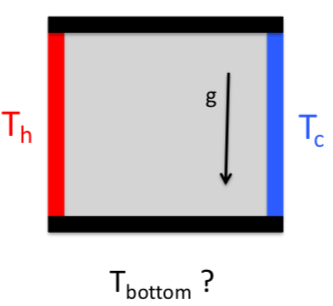
\includegraphics[width=0.75\textwidth]{./images/cavity_schematic}
  \caption{Schematic of density-driven cavity flow. The density of the fluid
    decreases with increasing temperature, and the walls are held at constant
    hot $T_h$ and cold $T_c$ temperatures. The resulting density gradients lead
    to an instability, which in turn drive fluid flow. The quantity we are
    interested in here is the temperature of the bottom wall.}
  \label{fig:cavity-schematic}
\end{figure}

The cavity of Figure \ref{fig:cavity-schematic} is filled with a fluid whose
density varies with temperature. Figure \ref{fig:density-linear} shows
experimental results in the form of intervals bounding the `true' values of the
density-temperature relation. The experimental data are compatible with a linear
relationship, and so one could fit a linear model to describe the
density-temperature relation. Since the experimental results are not fully
conclusive (they are given only as intervals), any linear model compatible with
the data is admissible. We will consider \emph{all} admissible linear models,
and their effect on the bottom wall temperature profile -- we do this via an
application of \emph{uncertainty propagation}, which we will discuss in Chapter
\ref{ch:wrangle}.

\begin{figure}[!ht]
  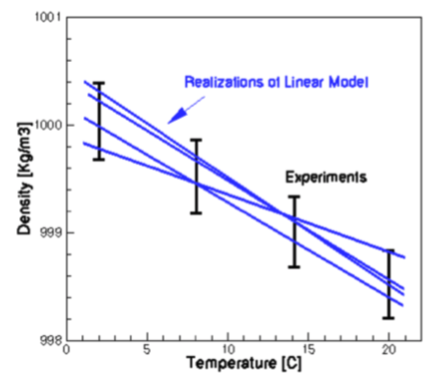
\includegraphics[width=0.75\textwidth]{./images/density_linear}
  \caption{Experimental intervals for temperature-density relation of cavity
    fluid. The data are compatible with a linear relationship, so we assume a
    family of linear models for the equation of state (EOS) -- informed by the
    data -- for uncertainty propagation. Each blue line is a \emph{realization}
    -- a particular instance -- of a density-temperature relation. We must
    consider the full ensemble of these relations in order to fully cover the
    space of possibilities implied by the interval data.}
  \label{fig:density-linear}
\end{figure}

Solving for steady-state behavior across all density-temperature relationships
yields a mean flow profile -- this is a single recirculation region, where hot
fluid rises near the left wall, and cold fluid falls near the right wall.

\begin{figure}[!ht]
  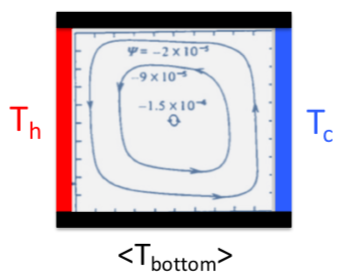
\includegraphics[width=0.80\textwidth]{./images/cavity_single}
  \caption{Mean streamfunction contours using the linear EOS assumption. These
    results show a single recirculation driving flow upward near the hot wall,
    and falling near the cold wall. (\textcolor{red}{TODO}: Re-generate; flip
    arrows)}
  \label{fig:cavity-single}
\end{figure}

One can compute maximum and minimum temperature values over all possible
(linear) density-temperature relationships and arrive at Figure
\ref{fig:bot-wall-single} -- the minimum and maximum values collapse to a single
curve. It happens that the mean flow field shown in Figure
\ref{fig:cavity-single} is the \emph{only} flow field possible in this setting.
However, this is not the full story.

\begin{figure}[!ht]
  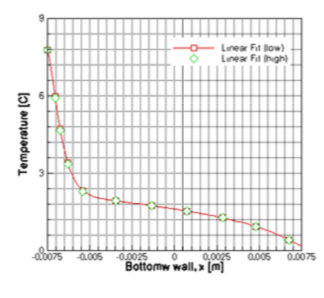
\includegraphics[width=0.75\textwidth]{./images/bot_wall_single}
  \caption{Bounds of bottom-wall behavior over all EOS models considered. Note
    that all the curves collapse. All the conditions considered result in
    \emph{the same} recirculation -- the uncertainty in our qoi is zero! If we
    stopped our analysis at this point, we would be \emph{confidently wrong}, as
    we will see below.}
  \label{fig:bot-wall-single}
\end{figure}

In truth, the density-temperature relationship is \emph{not linear}; the cavity
fluid is water, which undergoes a density \emph{inversion} near its freezing
point. This is the familiar behavior of floating ice.

\begin{figure}[!ht]
  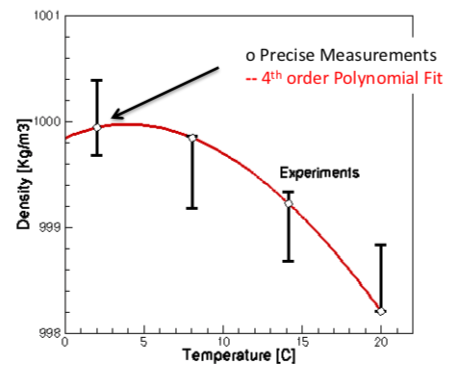
\includegraphics[width=0.75\textwidth]{./images/density_poly}
  \caption{Experimental intervals \emph{and point estimates} for
    temperature-density relation of cavity fluid -- the fluid is water, which
    undergoes a density inversion near freezing conditions. This slight
    nonlinearity has important ramifications for the flow field, which we
    consider in Figure \ref{fig:cavity-double}.}
  \label{fig:density-poly}
\end{figure}

Considering this polynomial density-temperature relation yields the behavior in
Figures \ref{fig:cavity-double} and \ref{fig:bot-wall-double}.

\begin{figure}[!ht]
  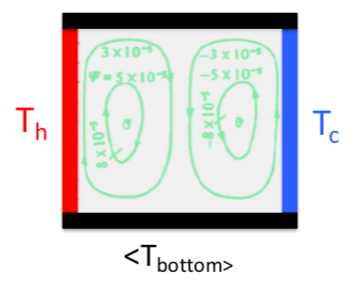
\includegraphics[width=0.75\textwidth]{./images/cavity_double}
  \caption{Streamfunction contours using the (single) polynomial EOS fit. These
    results show a pair of recirculation regions, which change the qualitative
    behavior significantly.}
  \label{fig:cavity-double}
\end{figure}

\begin{figure}[!ht]
  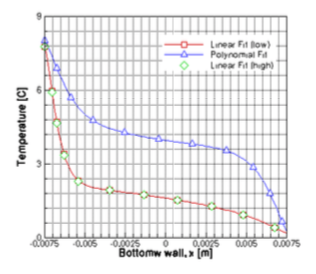
\includegraphics[width=0.75\textwidth]{./images/bot_wall_double}
  \caption{Bounds of bottom-wall behavior over all linear EOS models, and using
    the polynomial fit. We can see that the double-recirculation results in a
    considerably higher bottom-wall temperature -- hot fluid is transported to
    the middle of the bottom-wall via the double-recirculation, resulting in a
    generally hotter temprature profile.}
  \label{fig:bot-wall-double}
\end{figure}

\clearpage
The existence of a density inversion may seem obvious in retrospect, but the
truth is actually even more complicated. The precise temperature at which the
inversion occurs depends on the water salinity (Fig. \ref{fig:inversion-salt})
which will add additional complexity and uncertainty to the density-temperature
relation. Clearly, based on Figure \ref{fig:bot-wall-double}, a slight tweak to
this relationship can result in considerably different behavior. There are a
number of questions that remain with this problem: First, how can we quantify
the uncertainty in a \emph{function}? This issue around the density-temperature
relation is an example of \emph{model-form uncertainty}. Second, how precisely
do we \emph{propagate} uncertainty from the inputs to the output qoi? This is an
exercise in \emph{uncertainty propagation}.

\begin{figure}[!ht]
  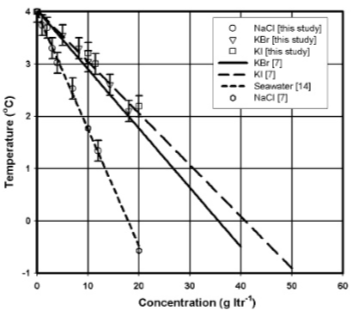
\includegraphics[width=0.75\textwidth]{./images/inversion_salt}
  \caption{Point of density inversion for water at different salinity
    concentrations.}
  \label{fig:inversion-salt}
\end{figure}

Answering the questions above is the aim of this primer! In what follows, we
will provide a tour through all the steps of managing uncertainty:

1. We will start by \textbf{formulating} our scientific or engineering problem.
This will involve standard things like building or selecting models, but also
identifying the level of precision one needs for the problem at hand, and
identifying different sources of uncertainty affecting the setting. This chapter
will introduce a number of foundational concepts, and a few tools for describing
uncertainty and simplifying problems.

2. We then \textbf{wrangle} the uncertainty, which involves forward and inverse
propagation. This is formally what researchers call \emph{uncertainty
  quantification}. This chapter will primarily focus on algorithms, as
propagation can be a very expensive proposition.

3. Finally, we will \textbf{act} upon the uncertainty, determining what -- if
any -- conclusions we can draw based on the results, and determining further
steps. Quantified uncertainties will help us to direct our attention to the most
pressing issues standing between us and a desired outcome. This chapter will
illustrate action primarily through examples.

\end{document}
